%%%%%%%%%%%%%%%%%%%%%%%%%%%%%%%%%%%%%%%%%
% Beamer Presentation
% LaTeX Template
% Version 1.0 (10/11/12)
%
% This template has been downloaded from:
% http://www.LaTeXTemplates.com
%
% License:
% CC BY-NC-SA 3.0 (http://creativecommons.org/licenses/by-nc-sa/3.0/)
%
%%%%%%%%%%%%%%%%%%%%%%%%%%%%%%%%%%%%%%%%%

%----------------------------------------------------------------------------------------
%	PACKAGES AND THEMES
%----------------------------------------------------------------------------------------

\documentclass{beamer}
\usepackage{multicol}
\usepackage{xcolor}
\usepackage{listings}

\definecolor{applegreen}{rgb}{0.55, 0.71, 0.0}
\definecolor{blue(ncs)}{rgb}{0.0, 0.53, 0.74}
\definecolor{burgundy}{rgb}{0.5, 0.0, 0.13}

\mode<presentation> {

\usetheme{CambridgeUS}

\usecolortheme{wolverine}

\definecolor{gold}{HTML}{D4A017}
\definecolor{darkgold}{HTML}{B7950B}

\setbeamercolor{palette primary}{bg=gold,fg=white}
\setbeamercolor{palette secondary}{bg=darkgold,fg=white}
\setbeamercolor{palette tertiary}{bg=black,fg=white}
\setbeamercolor{palette quaternary}{bg=gold,fg=white}

\setbeamercolor{frametitle}{bg=darkgold,fg=white}

\setbeamercolor{section number projected}{bg=black,fg=gold}
\setbeamercolor{item}{fg=black,bg=gold}
}

\usepackage{graphicx} % Allows including images
\usepackage{booktabs} % Allows the use of \toprule, \midrule and \bottomrule in tables

%----------------------------------------------------------------------------------------
%	TITLE PAGE
%----------------------------------------------------------------------------------------

\title[libCEED Finite Element Library]{Performance and Portability with\\the libCEED Finite Element Library} % The short title appears at the bottom of every slide, the full title is only on the title page

\author{Jeremy L Thompson} % Your name
\institute[CU Boulder] % Your institution as it will appear on the bottom of every slide, may be shorthand to save space
{University of Colorado Boulder \\ % Your institution for the title page
\medskip
\textit{jeremy.thompson@colorado.edu} % Your email address
}
\date{\today} % Date, can be changed to a custom date

\begin{document}

\begin{frame}
\titlepage % Print the title page as the first slide
\end{frame}

%------------------------------------------------

\begin{frame}
\begin{center}
\frametitle{Overview}

A global sparse matrix is no longer a good representation of a\\high-order linear operator\\

~\\

libCEED is an extensible library that provides a portable\\algebraic interface and optimized implementations\\

~\\

We have an example of portable and adaptable implementation with\\Navier-Stokes solver in libCEED and PETSc

~\\

We have results comparing performance on benchmark problems

\end{center}
\end{frame}
 
%------------------------------------------------

\begin{frame}
\frametitle{Overview} % Table of contents slide, comment this block out to remove it
\tableofcontents % Throughout your presentation, if you choose to use \section{} and \subsection{} commands, these will automatically be printed on this slide as an overview of your presentation
\end{frame}

%----------------------------------------------------------------------------------------
%	PRESENTATION SLIDES
%----------------------------------------------------------------------------------------

%------------------------------------------------
\section{Introduction}
%------------------------------------------------

\begin{frame}
\begin{center}
\frametitle{Assembled Matrix Cost}

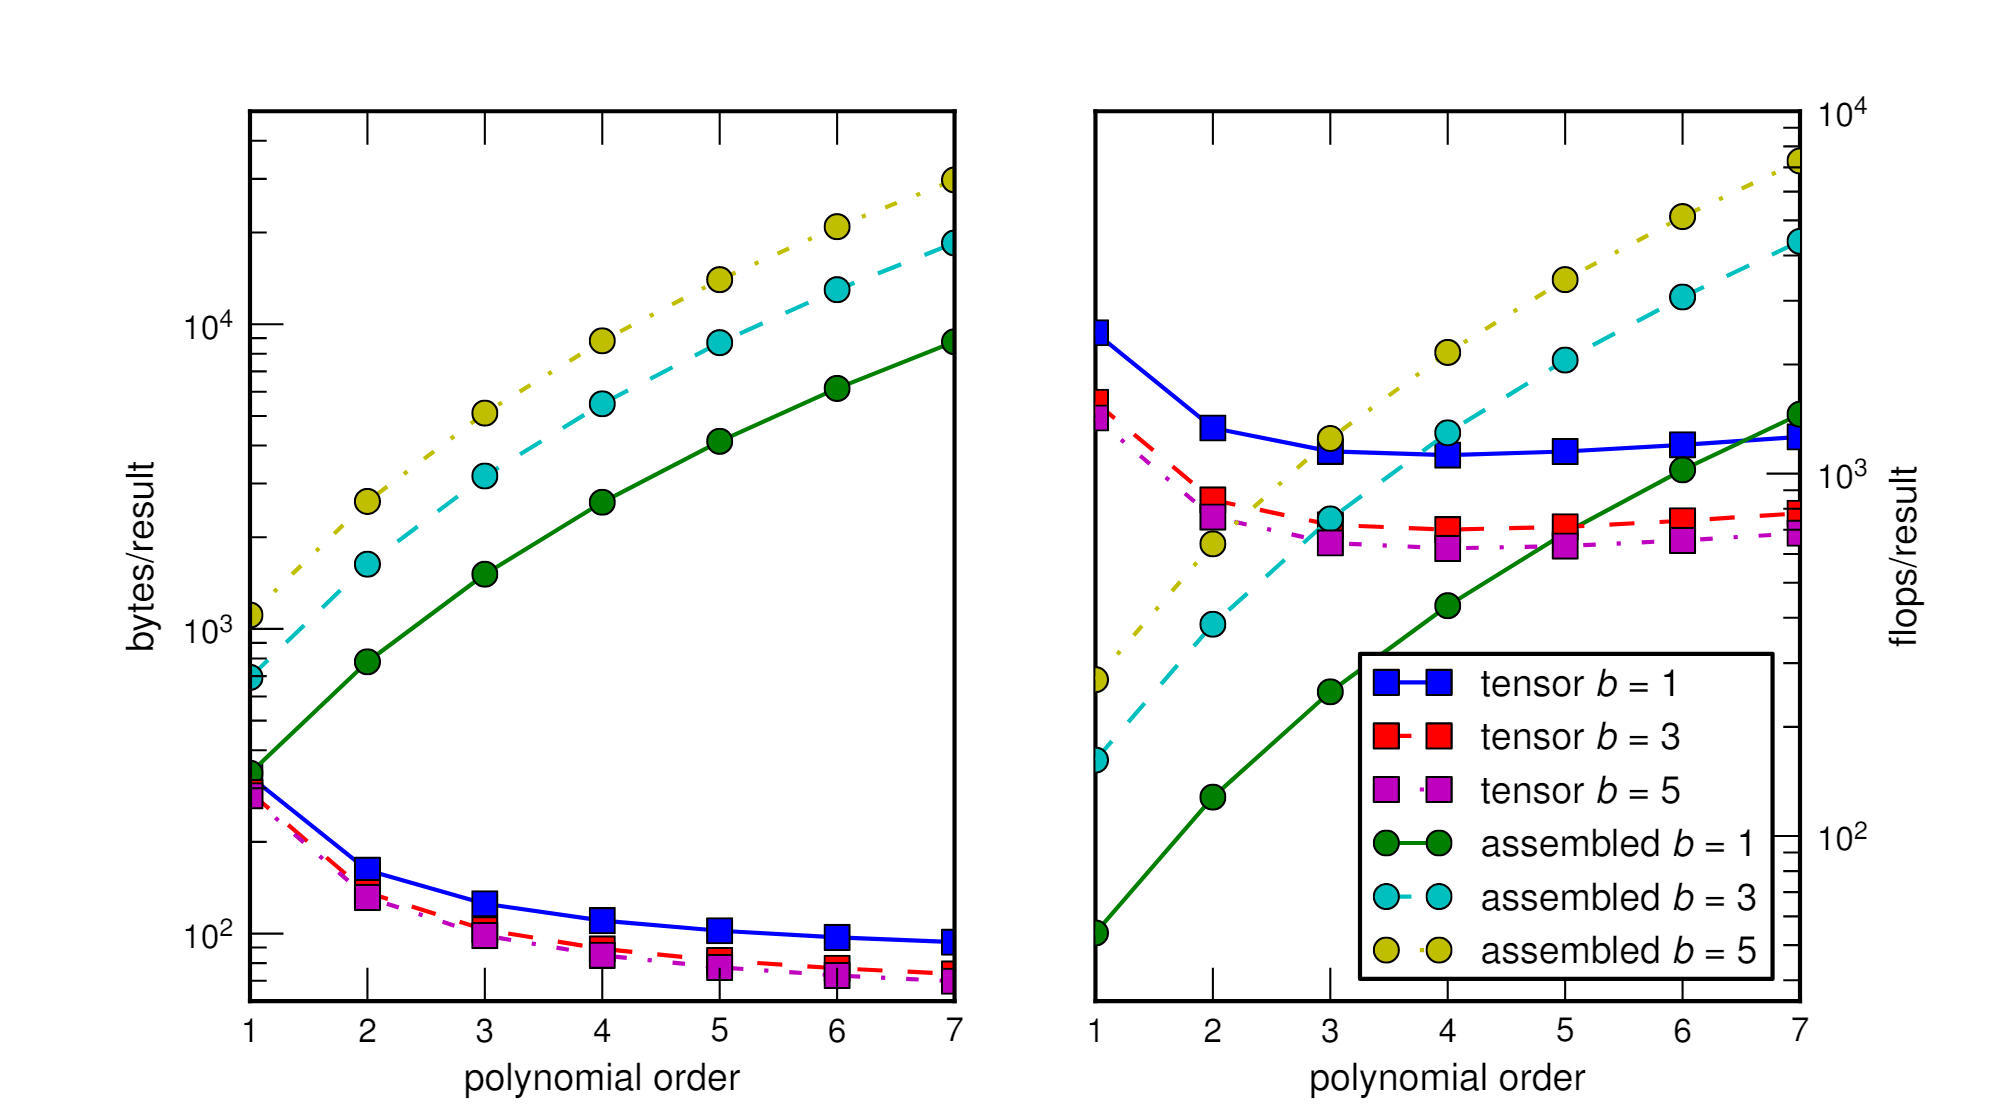
\includegraphics[height=5.5cm]{libCEEDtensorVsAssembled}

 Memory bandwidth and ops per dof to apply a Jacobian from $Q_k$ discretization of a $b$-variable PDE system using an assembled matrix versus matrix-free exploiting the tensor product structure

\end{center}
\end{frame}

%------------------------------------------------

\begin{frame}
\begin{center}
\frametitle{Matrix Free Implementation}

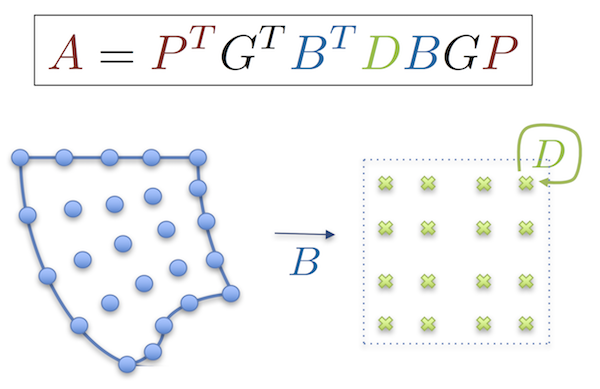
\includegraphics[width=5cm]{libCEEDRefElm}

\begin{itemize}

\item Avoid global matrix assembly

\item Map each element to reference element

\item All data computed on the fly or precompute static data

\item Easy to parallelize across nodes

\end{itemize}

\end{center}
\end{frame}

%------------------------------------------------
\section{libCEED}
%------------------------------------------------

\begin{frame}
\begin{center}
\frametitle{libCEED API}

\begin{itemize}

\item BSD-2 license, C99 library with F77 interface\\

~\\

\item Releases: v0.2 March and v0.3 (imminent)

~\\

\item Provides on-device operator implementation\\

~\\

\item Easy to incorporate into existing code\\

~\\

\item Supports multiple types of computational devices\\

\begin{itemize}

\item CPU - Reference and blocked, template for new backends

\item OCCA (jit) - CPU, OpenMP, OpenCL, and CUDA

\item MAGMA

\item CUDA (in final development)

\item One source code can call multiple CEEDs with different backends

\end{itemize}

\end{itemize}

\end{center}
\end{frame}

%------------------------------------------------

\begin{frame}
\begin{center}
\frametitle{Operator Decomposition}

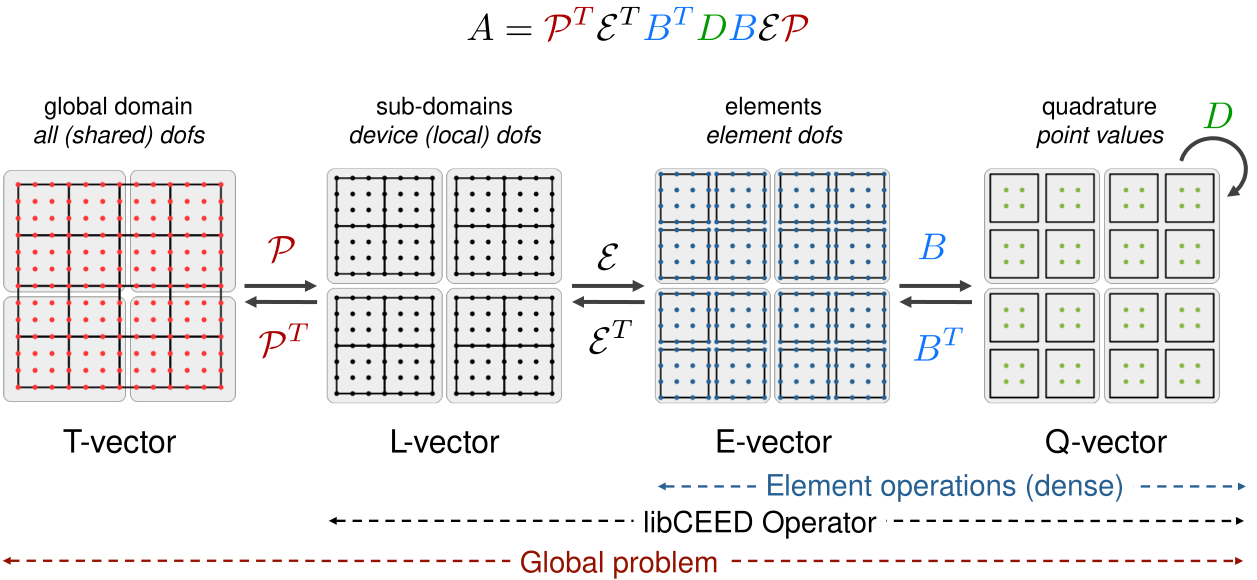
\includegraphics[width=11cm]{libCEEDAPI}

\end{center}
\end{frame}

%------------------------------------------------

\begin{frame}
\begin{center}
\frametitle{API Objects}

\begin{itemize}

\item $G$ - CeedRestriction\\

\hspace{6mm} Restrict to single element\\

\hspace{6mm} User choice in ordering\\

~\\

\item {\color{blue(ncs)} $B$} - CeedBasis\\

\hspace{6mm} Actions on basis such as interpolation,\\

\hspace{10mm} gradient, divergence, curl\\

\hspace{6mm} Independent of geometry\\

~\\

\item {\color{applegreen} $D$} - CeedQFunction\\

\hspace{6mm} Operator action at quadrature points\\

\hspace{10mm} to include coefficient functions\\

\hspace{6mm} Choice of when to compute metric terms and coefficents

\end{itemize}

\end{center}
\end{frame}

%------------------------------------------------

\begin{frame}
\begin{center}
\frametitle{Device Level Operator}

\begin{itemize}

\item $L = G^T {\color{blue(ncs)} B^T} {\color{applegreen} D} {\color{blue(ncs)} B} G$ - CeedOperator\\

~\\

\item libCEED objects are combined to create a CeedOperator\\

~\\

\item CeedOperator gives operator action for elements on device\\

~\\

\item User code responsible for communication between devices\\

\hspace{6mm} $A = {\color{burgundy} P^T} L {\color{burgundy} P}$

\end{itemize}

\end{center}
\end{frame}

%------------------------------------------------

\begin{frame}
\begin{center}
\frametitle{Quadrature Function}

$A u = F ( v, u ) = \int_\Omega v \cdot f_0 ( u, \nabla u ) + \nabla v \cdot f_1 (u, \nabla u)$\\

~\\

\hspace{6mm} $A u = {\color{burgundy} P^T} G^T {\color{blue(ncs)} B^T} {\color{applegreen} D} {\color{blue(ncs)} B} G {\color{burgundy} P} u$\\

~\\

\begin{itemize}

\item Quadrature function at the heart of the libCEED operator\\

\item Multiple inputs and outputs\\

\item Independent operations at quadrature points, ordering and number of elements not specified

\item Code will be implementation agnostic\\

\end{itemize}

\end{center}
\end{frame}

%------------------------------------------------
\section{Navier-Stokes}
%------------------------------------------------

\begin{frame}
\begin{center}
\frametitle{Navier-Stokes Formulation}

\begin{itemize}

\item Compressible Navier-Stokes\\

~\\

\item State variables: density, momentum, and total energy\\

~\\

\item Boundary conditions:\\

\hspace{6mm} momentum - no-slip, non-penetrating\\

\hspace{6mm} density, energy - reflecting\\

~\\

\item Initial conditions: Straka 1993\\

~\\

\item Mesh: Box domain with hexehedral mesh

\end{itemize}

\end{center}
\end{frame}

%------------------------------------------------

\begin{frame}
\begin{center}
\frametitle{Strategy}

\begin{itemize}

\item Implemented in PETSc and libCEED\\

~\\

\item Setup phase computes geometric factors (Jacobian) and initial conditions\\

~\\

\item Forward Euler for proof-of-concept version\\

~\\

\item Compact: $\sim 480$ lines of PETSc code and $\sim 200$ lines of quadrature functions

\end{itemize}

\end{center}
\end{frame}

%------------------------------------------------

\begin{frame}[fragile]
\begin{center}
\frametitle{Navier-Stokes QFunction}

{\tiny
\begin{lstlisting}[language=C]
static int NS(void *ctx, CeedInt Q,
              const CeedScalar *const *in, CeedScalar *const *out) {
  // Inputs
  const CeedScalar *q = in[0], *dq = in[1], *qdata = in[2], *x = in[3];
  // Outputs
  CeedScalar *v = out[0], *vg = out[1];
...
  // Quadrature Point Loop
  for (CeedInt i=0; i<Q; i++) {
    // Setup
...
    // The Physics

    // -- Density
    // ---- u rho
    vg[i+(0+5*0)*Q] = rho*u[0]*BJ[0] + rho*u[1]*BJ[1] + rho*u[1]*BJ[2];
    vg[i+(0+5*1)*Q] = rho*u[0]*BJ[3] + rho*u[1]*BJ[4] + rho*u[1]*BJ[5];
    vg[i+(0+5*2)*Q] = rho*u[0]*BJ[6] + rho*u[1]*BJ[7] + rho*u[1]*BJ[8];

    // -- Momentum
...
    // -- Total Energy
    // ---- (E + P) u
    vg[i+(4+5*0)*Q]  = (E + P)*(u[0]*BJ[0] + u[1]*BJ[1] + u[2]*BJ[2]);
    vg[i+(4+5*1)*Q]  = (E + P)*(u[0]*BJ[3] + u[1]*BJ[4] + u[2]*BJ[5]);
    vg[i+(4+5*2)*Q]  = (E + P)*(u[0]*BJ[6] + u[1]*BJ[7] + u[2]*BJ[8]);
...
\end{lstlisting}
}

\end{center}
\end{frame}

%------------------------------------------------
\section{Benchmarks}
%------------------------------------------------

\begin{frame}
\begin{center}
\frametitle{Bakeoff Problems}


\includegraphics[height=1.5cm]{libCEEDCURCLogo}

\begin{multicols}{2}

\hspace{2mm} CEED Benchmark Problem 1\\

Problem: $\int v u = \int v f$ - $L^2$ projection\\

\hspace{2mm} CEED Benchmark Problem 3\\

Problem: $\int v \Delta u = \int v f$ - Poisson\\

\end{multicols}

~\\

\begin{flushleft}

\begin{multicols}{2}

Domain: 3D Cube\\

Elements: Hexahedral\\

Shape Function Order: $2$-$10$\\

Quadrature Points: $4^3$-$12^3$\\

Machine: CU Boulder Summit\\

~\\

Nodes: 1\\

CPUs: Intel Xeon ''Haswell''\\

Processors: 24 (12 used)\\

Compiler: Intel/17.4\\

MPI: Intel/17.3\\

~\\

\end{multicols}

\end{flushleft}

\end{center}
\end{frame}

%------------------------------------------------

\begin{frame}
\begin{center}
\frametitle{BP1}

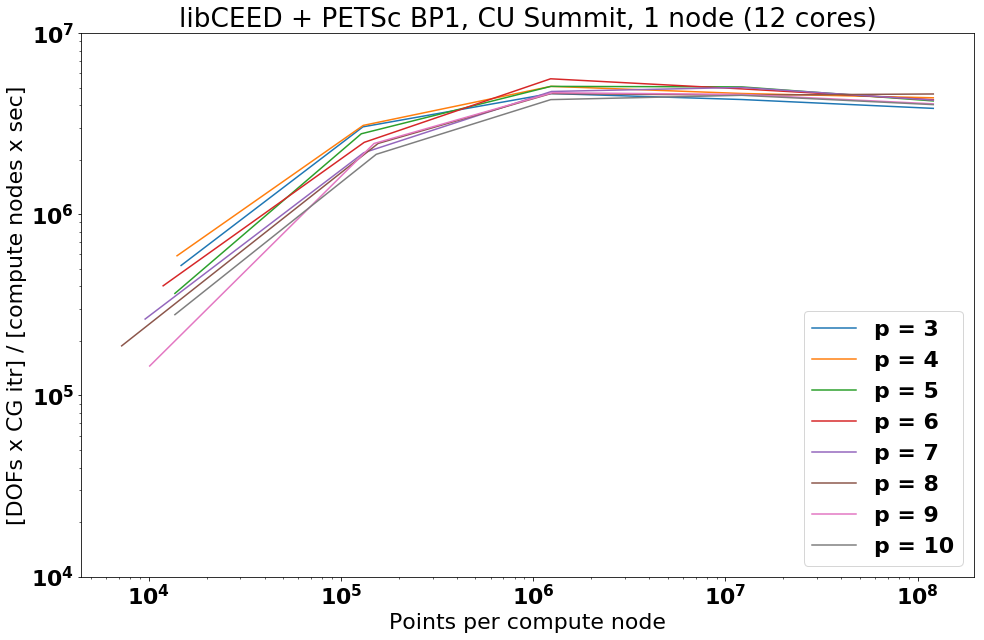
\includegraphics[width=10cm]{libCEEDPETScBP1}

* Disclaimer - Results are very 'muddy'; Host code is not fully optimized and timing is for entire host code, with setup and destruction *

\end{center}
\end{frame}

%------------------------------------------------

\begin{frame}
\begin{center}
\frametitle{BP3}

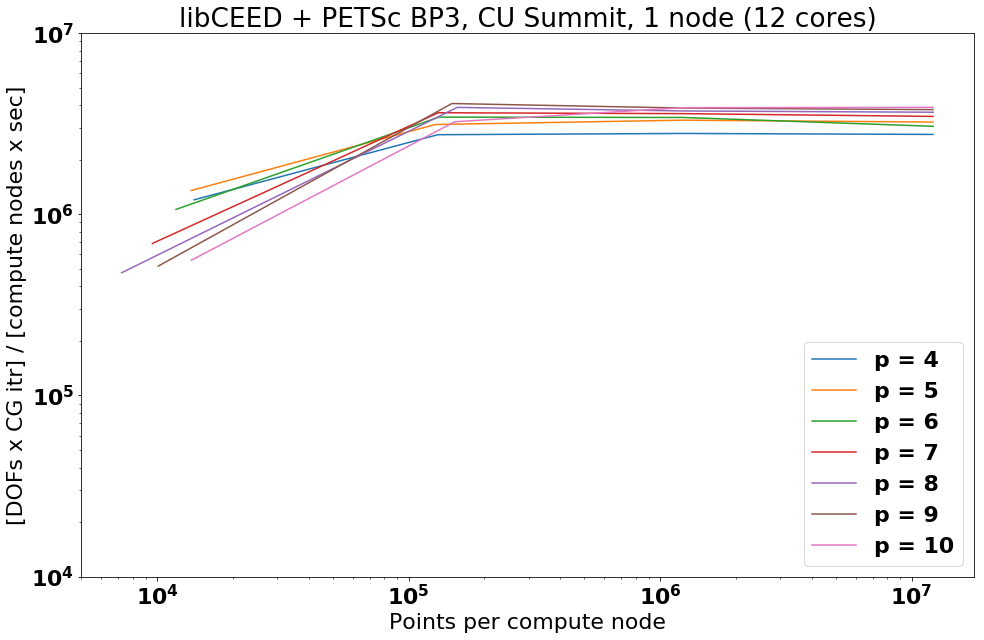
\includegraphics[width=10cm]{libCEEDPETScBP3}

* Disclaimer - Results are very 'muddy'; Host code is not fully optimized and timing is for entire host code, with setup and destruction *

\end{center}
\end{frame}

%------------------------------------------------

\begin{frame}
\begin{center}
\frametitle{MFEM}

\centerline{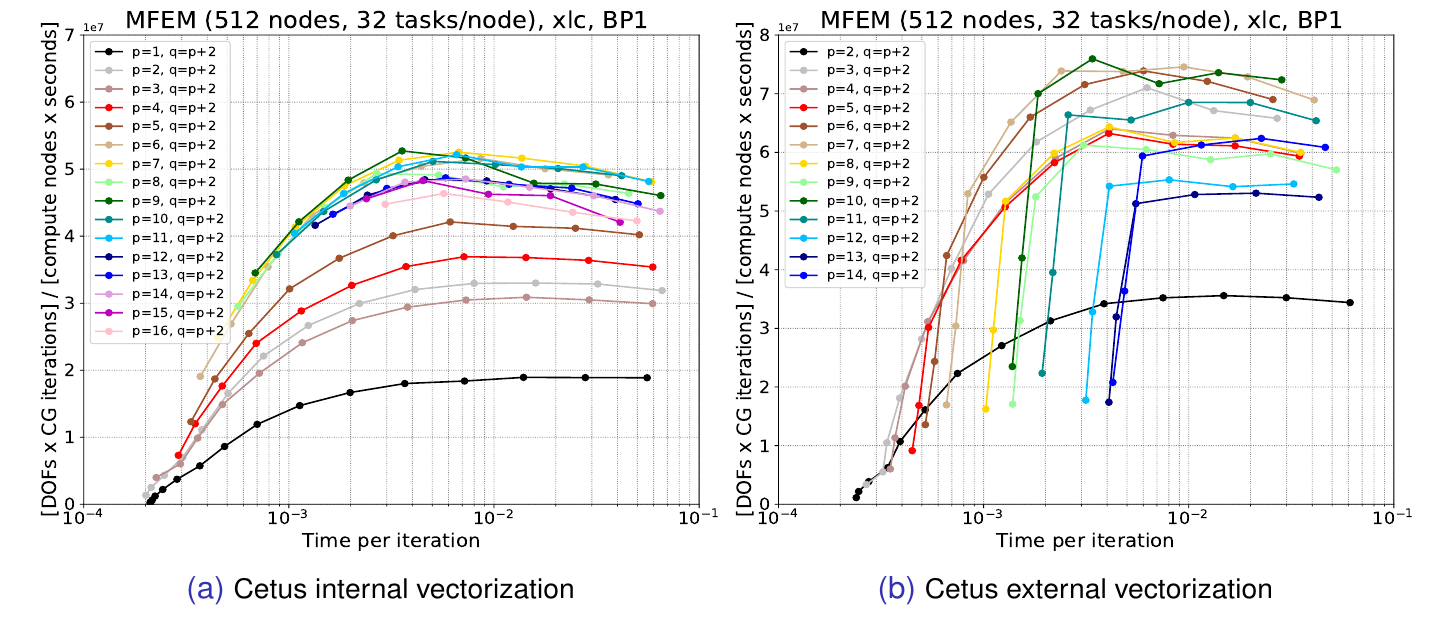
\includegraphics[width=12.5cm]{libCEEDMFEMBenchmarks}}

Results by Thilina Rathnayake

\end{center}
\end{frame}

%------------------------------------------------

\begin{frame}
\begin{center}
\frametitle{OCCA on Summit}

\centerline{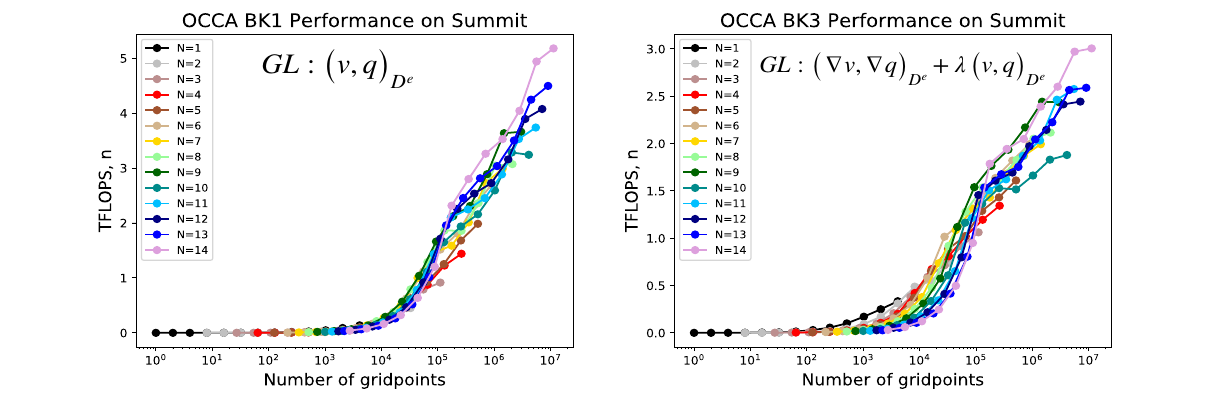
\includegraphics[width=14cm]{libCEEDOCCABenchmarks}}

Results by Thilina Rathnayake

\end{center}
\end{frame}

%------------------------------------------------

\begin{frame}
\begin{center}
\frametitle{Future Work}

\begin{itemize}

\item Continue performance tuning\\

\item Improve GPU backends, reduce data movement\\

\item Finalize pure CUDA backend\\

\item Optimize additional geometries: tets, pyramids, and prisms\\

\item Implement non-conforming meshes\\

\item Create library of user quadrature functions\\

\item Algorithmic differentiation of quadrature functions\\

\item Composite operators, for mixed meshes and multiphysics\\

\item Contributors and friendly users welcome

\end{itemize}

\end{center}
\end{frame}

%------------------------------------------------
\section{Questions}
%------------------------------------------------

\begin{frame}
\begin{center}
\frametitle{Questions?}

{\flushleft

Advisor: \hspace{8mm} Jed Brown\textsuperscript{1}\\

~\\

Collaborators: Valeria Barra \textsuperscript{1}, Jean-Sylvain Camier\textsuperscript{2}, Tzanio Kolev\textsuperscript{2},\\
\hspace{23mm} Veselin Dobrev\textsuperscript{2}, Tim Warburton\textsuperscript{3}, David Medina\textsuperscript{4},\\
\hspace{23mm} \& Thilina Rathnayake\textsuperscript{5}\\

~\\

Grant: \hspace{11mm} Exascale Computing Project (17-SC-20-SC)\\

~\\

~\\

\small{1: University of Colorado, Boulder\\
2: Lawrence Livermore National Laboratory\\
3: Virginia Polytechnic Institute and State University\\
4: OCCA\\
5: University of Illinois, Urbana-Champaign\\}}

\end{center}
\end{frame}

%------------------------------------------------

\begin{frame}[noframenumbering]
\titlepage % Print the title page
\end{frame}

%------------------------------------------------

%----------------------------------------------------------------------------------------

\end{document}
